\documentclass[aps,prl,superscriptaddress,12pt]{revtex4-1}
	\usepackage{graphicx}  % needed for figures
	\usepackage{fancyhdr} % needed for team number and page number
	\usepackage{amsmath}
	\usepackage{comment}
	% configure desired header format
	\pagestyle{fancy}
	\fancyhf{}
	\lhead{ Team \#  }
	\rhead{ Page \thepage\text{ }of \pageref{LastPage} }

\begin{document}

	\title{Macroscopic and Microscopic Assessment of Traffic Rules}
	%\author{Abigail Chua}
	%	\affiliation{Denison University, Granville, OH, 43023, USA}
	%\author{Yubo Yang}
	%	\affiliation{Denison University, Granville, OH, 43023, USA}
	%\author{Yifu Zhao}
	%	\affiliation{Denison University, Granville, OH, 43023, USA}
		
	\begin{abstract}
		Summary goes here
	\end{abstract}
	
\maketitle

	\section{Interpretation of the Problem}


	\section{Model}
	To simplify the model, we consider a stretch of straight two-lane freeway with no on/off ramp. To assess the performance of the given traffic rule, we would like to analyze its impact on traffic flow, road safety, and ability to recovery from traffic jams.
		\subsection{Traffic Flow} 
		\begin{table}[h]
	\begin{tabular}{|c|c|c|} \hline
	quantity & variable & unit \\ \hline
	traffic density on lane 1 & $\rho_1$ & cars/m \\ \hline
	traffic density on lane 2 & $\rho_2$ & cars/m \\ \hline
	equilibrium velocity on lane 1 & $v_1$ & m/s \\ \hline
	equilibrium velocity on lane 2 & $v_2$ & m/s \\ \hline
	\end{tabular}
	\caption{ variables used in the macroscopic model \label{tab:variables} }
	\end{table}	 
	Traffic flow rate is best captured in a macroscopic model with variables shown in Table \ref{tab:variables}. The total amount of traffic flow will then be determined by
	\begin{align}
	& Q(\rho_1,\rho_2) = \rho_1\cdot v_1(\rho_1,\rho_2)+\rho_2\cdot v_2(\rho_1,\rho_2) & \label{eq:flow}
	\end{align}
	
	We further assume that at equilibrium, there is some velocity-density relation. Given this velocity-density relation, the flow at any given junction of the freeway at a given time is completely determined by the local traffic densities $\rho_1$ and $\rho_2$.
	
	\begin{comment} 
Kerner elt. al. proposed the following relationship in 2002. 
	\begin{align}
	& v_e = v_o\left( (\frac{1+e^{\rho/\rho_m-0.25}}{0.06})^{-1} - 3.76\times10^{-6} \right) & \label{eq:Kerner}
	\end{align}
	It captures the key 
	\begin{figure}
	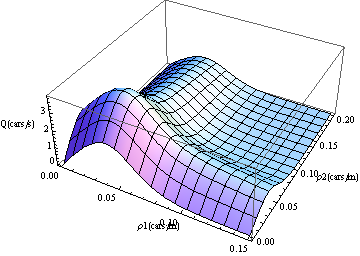
\includegraphics[scale=1]{plot/Q_p1_p2}
	\caption{equilibrium traffic flow as a function of traffic densities using Kerner's velocity-density relation\label{fig:Q_p1_p2}}
	\end{figure}
	\end{comment}
	
	To derive such a relation, we consider all cars to have uniform length $l(m)$, travel with uniform velocity $v_e(\rho)$ and maintain uniform bumper-to-bumper distance $d(m)$ from their neighbors. At this equilibrium, each car will take up a total space of $d+l$ on one lane of the freeway. Since the highway won't be completely conjested all the time, there will normally be extra free space in between cars in addition to the safe following distance. We can think of this free space as being filled by an invisible vihcle density $\rho_0$, therefore
	\begin{align}
	& \rho + \rho_o= \frac{1}{d+l} & \label{eq:follow}
	\end{align}
	Incorporating the two-second rule enforced by the New York Sate Department of Motor Vehicles \cite{science_writing}, $d=v_e(\rho)t$, where $t=2s$. Equation (\ref{eq:follow}) can be solved to obtain and expression for $v_e(\rho)$
	\begin{align}
	& v_e(\rho) =  (\frac{1}{\rho+\rho_o}-l)/t& 
	\end{align}
	We define the capacity (or jamming density) of the road by the density at which traffic stops flowing
	\begin{align}
	& 0 =  (\frac{1}{\rho_j+\rho_o}-l)/t & \\
	\Rightarrow & \rho_j=\frac{1}{l}-\rho_o &
	\end{align}
	This speed-density relationship also imposes a natural speed limit on the road, specifically the speed of traffic at zero density
	\begin{align}
	& v_{nl} = v_e(0) =  (\frac{1}{\rho_o}-l)/t &
	\end{align}
	Consider the natural speed limit of a freeway lane to be $50m/s$, about $110mph$ then $\rho_o=\frac{1}{105}$ and $\rho_j=0.19$
	\begin{figure}[h]
	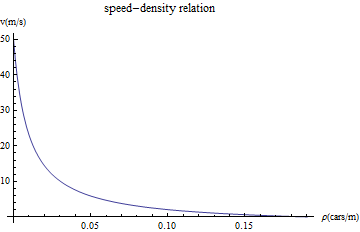
\includegraphics[scale=.6]{plot/speed_density}
	\caption{speed-density relation with a natural speed limit of $50m/s$}
	\end{figure}
	
	With the speed-density relation determined, we can derive the flow of a two-lane freeway using the prescription described in equation \ref{eq:flow}
	\begin{figure}
	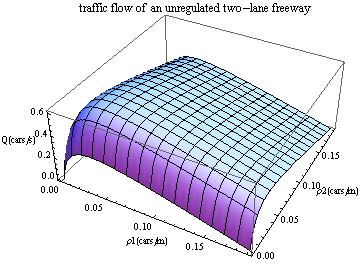
\includegraphics[scale=.6]{plot/unregulated_flow}
	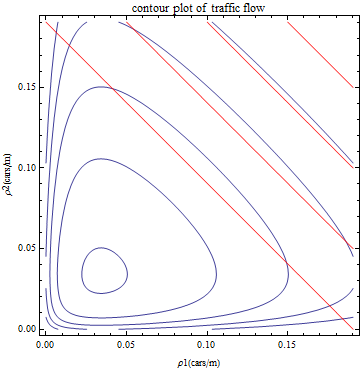
\includegraphics[scale=.45]{plot/contour_flow}
	\caption{traffic flow as a function of lane 1 and lane 2 traffic density on a two-lane freeway}
	The contour plot provides a good prediction for how the traffic rule might affect the amount of traffic flow. In light traffic, $\rho_1+\rho_2$ is small. As seen in the bottom left corner of the contour plot of traffic flow, any bias in one lane over the other will reduce traffic flow. In this regime, as traffic increase, vehicles should utilize both lanes in the same way to maximize the total amount of traffic flowing through the freeway. However, as traffic satuate the road capacity, bias in the densities of the the roads does not affect traffic flow in a significant manner. This is demonstrated in the contour plot through an overlap of the contours lines of flow(blue) and of total traffic(red) on the road.
	\end{figure}
	
		\subsection{Traffic Disturbance}
		An important measure of the robustness of a traffic rule is its ability to resolve traffic disturbance. Here we adopt a hybrid of car-following and classic kinematic wave theory from literature \cite{tang_2004}.  In this theory, classic LWR kinematcs wave model \cite{lighthill_1955,richards_1955} is combined with a variation of car-following theory \cite{jiang_2002}, giving the following four equations that describe the temperal and spatial variations of the traffic density as well as average velocity of vehicles on the two lanes of the freeway.
	\begin{align} \label{eq:pde}
	& \frac{\partial \rho_1}{\partial t} + \frac{\partial \rho_1}{\partial x}v_1+\rho_1\frac{\partial v_1}{\partial x}=s_1 & \\
	& \frac{\partial v_1}{\partial t} + v_1\frac{\partial v_1}{\partial x} = \frac{v_{1e}-v_1}{\tau_1}+c_{10}\frac{\partial v_1}{\partial x} & \\
	& \frac{\partial \rho_2}{\partial t} + \frac{\partial \rho_2}{\partial x}v_2+\rho_2\frac{\partial v_2}{\partial x}=s_2 & \\
	& \frac{\partial v_2}{\partial t} + v_2\frac{\partial v_2}{\partial x} = \frac{v_{2e}-v_2}{\tau_2}+c_{20}\frac{\partial v_2}{\partial x} &
	\end{align}
	where we take $v_{1e} = v_{2e}$ to be the equilibrium velocity-density relations derived from previous sections (equation (\ref{eq:ve})). Adhering to the assumption that the two roads are identical, we choose $\tau_1=\tau_2=10s$ and $c_{10}=c_{20}=11m/s$ according to the stability contraint proposed by Tang and Huang\citep{tang_2004}.
	
	We impose periodic boundary condition and initial condition that represents a traffic disturbance in lane 1 to observe traffic behavior after the disturbance. $\rho_1(x,0)$ is the functional form of a traffic disturbance suggested in \citep{tang_2004}. $L$ is the length of freeway of interest. $\rho_{10}$ is the average vehicle density on lane 1 and $\Delta \rho_{10}$ is the size of the disturbance. 
	\begin{align}
	& \rho_1(0,t) = \rho_1(L,t) & \\
	& v_1(0,t) = v_1(L,t) & \\
	& \rho_2(0,t) = \rho_2(L,t) & \\
	& v_2(0,t) = v_2(L,t) & \\
	&\rho_1(x,0)=\rho_{10}+\Delta \rho_{10}\left(  cosh^{-2}(\frac{160}{L}(x-\frac{5L}{16}))-\frac{1}{4}cosh^{-2}(\frac{40}{L}(x-\frac{11L}{32})) \right)& \\
	& v_1(x,0) = v_{1e}(\rho_1(x,0)) & \\
	&\rho_2(x,0)= \rho_{20}& \\ \label{eq:ic}
	& v_2(x,0) = v_{2e}(\rho_2(x,0)) & \\
	\end{align}
	
	The source terms for lane 1 and lane 2 must satiesfy  $s_1+s_2=0$ by the assumption of no on/off ramp. By changing these source terms, we are effectively putting different traffic rules into effect. For example, $s_1=0$ correspond to the rule that no vehicle is allowed to switch lanes, whereas $s_1= \rho_2-\rho_1$ enforces the rule that vehicles are only allowed to switch from lane 1 to lane 2 if the car density on lane 2 is lower than that on lane 1. Here we adopt the rule $s_1=\rho_2/\rho_{20}-\rho_1/\rho_{10}$. The addition of $\rho_{10}$ and $\rho_{20}$, the equilibrium densities for the two lanes, allows us to bias the utilization of the two roads. Specifically, if the keep-right rule is enforced (and suppose lane 2 is the overtaking lane), then vehicles on lane 2 must generally have faster speed than those on lane 1, therefore by the reciprocal velocity-density relation (equation \ref{eq:ve}) we can imply $\rho_{10}>\rho_{20}$.
		
	Recall that the equilibrium velocity-density relation (equation \ref{eq:ve}) produces a natural speed limit of $50$ m/s and a jaming density of $\rho_j=0.19$ cars/m. This provides us with a guideline for the overall scale of equilibrium traffic for light and heavy conditions. For the fair comparison, the total number of cars on the road is supposed to be the same for the case with no rule enforced and the case with the keep-right rule. For light traffic we chose $\rho_{10}+\rho_{20}=0.06 \approx \frac{1}{3}\rho_j$ whereas for heavy traffic we chose $\rho_{10}+\rho_{20}=0.24 \approx \frac{5}{4}\rho_j$
	Equations (\ref{eq:pde}-\ref{eq:ic}) are solved using Mathematica 9.0. Four sets of parameters were chosen to represent
	\begin{enumerate}
	\item{light traffic, no rule:}
		$\rho_{10}=\rho_{20}=0.03, \Delta \rho_{10}=0.001$
		\begin{figure}[h]
		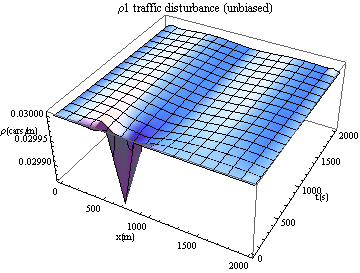
\includegraphics[scale=.6]{plot/p1_light_disturb_unbiased}
		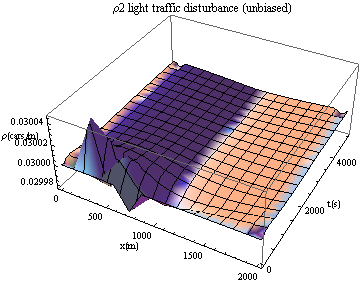
\includegraphics[scale=.6]{plot/p2_light_disturb_unbiased}
		\end{figure}
	\item{light traffic, keep-right:}
		$\rho_{10}=0.045, \rho_{20}=0.005, \Delta \rho_{10}=0.001$
		\begin{figure}[h]
		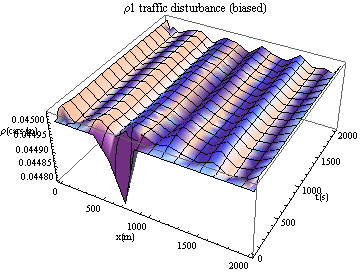
\includegraphics[scale=.6]{plot/p1_light_disturb_biased}
		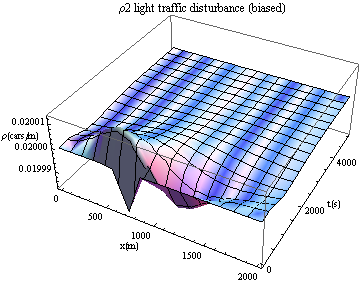
\includegraphics[scale=.6]{plot/p2_light_disturb_biased}
		\end{figure}
	\item{heavy traffic, no rule:}
		$\rho_{10}=\rho_{20}=0.12, \Delta \rho_{10}=0.001$
		\begin{figure}[h]
		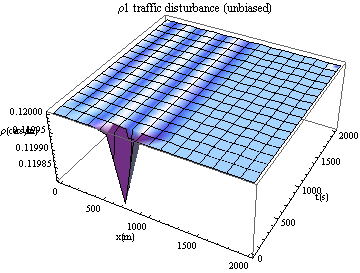
\includegraphics[scale=.6]{plot/p1_heavy_disturb_unbiased}
	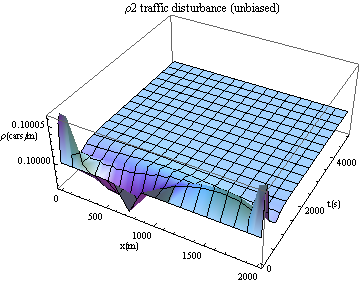
\includegraphics[scale=.6]{plot/p2_heavy_disturb_unbiased}
		\end{figure}
	\item{heavy traffic, keep-right:}
		$\rho_{10}=0.19, \rho_{20}=0.05, \Delta \rho_{10}=0.001$
		\begin{figure}[h]
		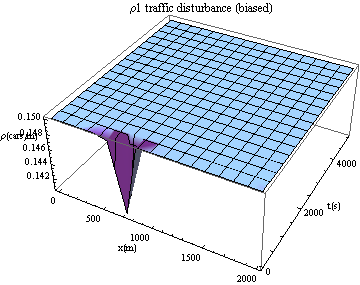
\includegraphics[scale=.6]{plot/p1_heavy_disturb_biased}
		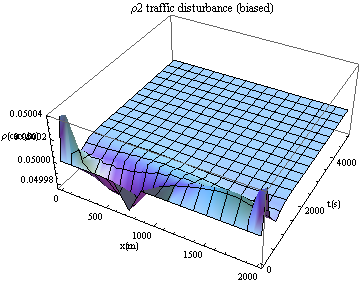
\includegraphics[scale=.6]{plot/p2_heavy_disturb_biased}
		\end{figure}
	\end{enumerate}
	Under light traffic conditions, having no rule actually helps the stability of traffic, a slight disturbance in one lane does not cuase lasting disturbance, whereas when the keep-right rule is enforced, lasting disturbance, even though very slight, will survive.	
	
	Under heavy traffic conditions, on the other hand, reverese the situation. Having the keep-right rule dramatically increases the stability of traffic against a slight disturbance.	
	
		\subsection{Safety}
		We used a similar microscopic model with two lanes to examine the safety issue. There are a few different criteria that could be used to determine the safety. In our model, we consider mainly the two following, total amount of slow down distance by all affected cars and the number of cars that need to slow down. 

\subsubsection{Assumption of safety analysis}

Before analyzing the model, there are a few assumptions that we have made to simplify the model. Firstly, we assume each vehicle is a particle, so the length is negligible. Secondly, to analyze the road performance of the cars with different traveling speed, we assume that the cars have two types of speed, $v_1$ and $v_2$ with $v_2 > v_1$. In a traveling equilibrium of a lane, we assume that the cars are separated by a distance of $d$ that is related to the speed,$v$, of the car on that lane , following time, $t$, and the traffic density on that lane, $\rho$. In particular, since cars are traveling in equilibrium condition, the speed is constant (except those cars that want to overtake others). The following time $t$ refers to the safe time difference that drivers assume for two adjacent cars to pass through the same spot of the road, which is usually around $1$ to $2$ seconds. Therefore, drivers will keep at least $d_m = vt$ distance from the car in front. However, usually drivers will not stick to the distance $d_m = vt$, but rather keep a distance that is a little bit further for extra safety. Hence, in equilibrium, the actual difference between two cars is $d_s = vt + d_0$, where $d_0$ is the extra safety distance, and it is a function of lane traffic density $\rho$, thus $d_0 = f(\rho)$. According to our previous analysis, $d_0$ has a inverse relationship with $\rho$, i.e. when $\rho$ is low, $c$ is large.

\subsubsection{Analysis of safety model on both ruled and unruled traffic}

We then consider the performance difference between the two situations (one with rule applied and one without). First consider the case where drivers are free to drive on both left and right lane, which is the case where no rule is enforced. In this case, when a car, $C_0$, overtakes another one, it needs to shift to the other lane and push back cars on that lane (see figure \ref{safety1}). In particular, in order to keep at least a safe distance $d_m = vt$ from the previous car, $C_0$ has to slow down and until the difference with the front car is $d_m$. This will suppress the distance with the car behind $C_1$, which will cause the car to slow down as well. Therefore, the action of overtaking will cause a series of slowing down of cars until all have reached at least a minimum safety distance $d_m$. 

\begin{figure}
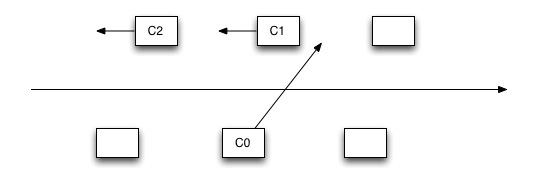
\includegraphics[scale = 0.5]{plot/P1}
\caption{car overtaking illustration of unruled two lane traffic\label{safety1}}

\end{figure}

\begin{figure}
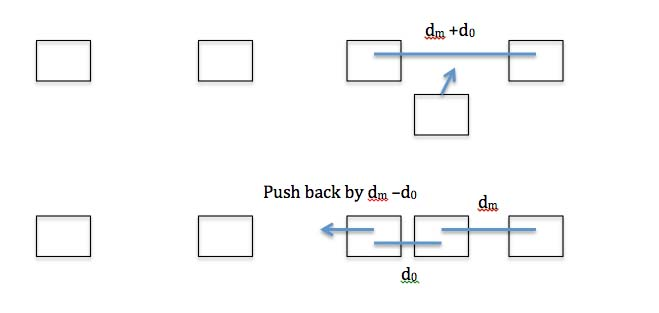
\includegraphics[scale = 0.5]{plot/P2}
\caption{illustration of minimum distance pushed back\label{safety2}}
\end{figure}

From the graphical illustrations(\ref{safety2}), we notice that the car $C_0$ is pushed back by $d_m-d_0$, $C_1$ is pushed back by $d_m-2d_0$ and the $i^{th}$ car is pushed back by $d_m-id_0$. The car $C_i$ will not slow down if $d_m-id_0\le 0$, i.e. $d_m \le id_0$. Therefore, the number of cars slowed down $n \approx d_m/d_0$ when $d_0 << d_m$. 

Thus, we would be able to calculate the total amount of braking distance made by all cars after $C_0$

\begin{align}
&d_t = d_m-d_0 + d_m-2d_0 + \dots + d_m - nd_0 & \\
&d_t = nd_m-\frac{(d_0+nd_0)(n)}{2}&\\
&d_t = \frac{d_m^2}{d_0}-\frac{(d_0+d_m)(d_m)}{2d_0}&\\
&d_t = \frac{d_m^2-d_0d_m}{2d_0}
\end{align}

In particular, if the $d_t \le 0$, i.e. no car needs to slow down, we have $d_m\le d_0$, which means that when the minimum safe distance is less than the extra safe distance, no car will slow down. 

Now, let's take a look at the case if the rule is applied to the two lane traffic situation. In this case, the right lane is the regular lane and the left lane is the passing lane, which suppose to have a higher speed. When a car, $C_0$, is trying to take over the car(s) in front, it needs to shift to the left lane and then shift back to the right lane after overtaking a number of cars. Suppose $C_0$ only overtake one car $C_1$, then when $C_0$ shifts back to the right lane, $C_1$ probably needs a slow down if $d_m>d_0$. However, we notice that because $C_0$ has shifted out of the right lane in the first place, it has left a space of $2(d_s)$ behind $C_1$. Thus, the slow down distance of $C_1$ after $C_0$ has shifted back to the is $d_m-d_0$. Therefore, the distance remain behind $C_1$ after it finished slowing down is

\begin{align}
&2(d_s)-(d_m-d_0)&\\
=\ &2(d_m+d_0)-(d_m-d_0)&\\
=\ &d_m+3d_0&\\
\ge \ &d_m&
\end{align}

Therefore, in this case, $C_1$ is the only affected car. And the slow down distance is $d_m-d_0$

If we increase the number of car that $C_0$ overtakes, we know that the first car overtaken by $C_0$ needs to slow down by $d_m-id_0$, which is less than $d_m+3d_0$. Thus, the maximum number of cars affected is $max(d_m/d_0, i)$. This shows that the number of cars slowed down is no more than the previous case. In addition, the total amount of slow down distance is still

\begin{equation}
d_t = d_m-d_0 + d_m-2d_0 + \dots + d_m - id_0 
\end{equation}
However, since $i\le n$, the total slow down distance is less or equal to the previous case. 


\subsubsection{Safety model on light and heavy traffic comparison}

Now, let's consider the difference between light and heavy traffic. From our assumption, as the traffic density $\rho$ increase, $d_0$ decrease. Therefore, the number of cars slowed down $n\approx d_m/d_0$ is increased. This explains that as the traffic become heavier, the chance for a safety risk is increased. In light traffic, we notice that $d_m \approx d_0$, and then in this case, both situation (ruled and unruled) has no need for slowing down. Thus, the difference in safety issue is insignificant. 


\subsubsection{summary of safety}

In analyzing the safety issue, we used a similar microscope model to determine the relationship between adjacent cars. This is built upon a discreet realization of the kinematic model to simulate and calculate the situation of overtaking in both ruled and unruled traffic. We were able to draw the conclusion that the ruled traffic is better at reducing the safety threat.

\subsubsection{Issue with compliance}

In the previous safety model, we assumed that each one follow the suggested rule by setting the following time $t = 2$ and  the minimum following distance $d \ge vt$. However, in case of low compliance, some people may shorten the following time, thus the following distance. Suppose those cars has a shorter following distance $d_m'$. Because of their lowered following time, the distance between it and the car in front is almost inflexible. Thus, the wave of slowing down would not be tolerant at those cars. The number of cars involved in wave of slowing down would be $n' = d_m/d_0+\alpha$, where $\alpha$ is the number of cars that has shorter following distance $d_m'$. This increase in number of slowing down cars is a potential risk to the safety issue. 
	
	\section{Discussion}
		\subsection{Compliance}
		All previous analysis is conducted based on the assumption that everyone is compliant with the rules. To test the effect of noncompliant drivers, we reconsider the velocity-density relation. Suppose a fraction $\eta$ of the drivers do not follow the two-second following rule. Instead they keep a different separation time $t'$. In this case equation (\ref{eq:follow}) needs to be modified to 
\begin{align}
& (1-\eta)(\rho + \rho_o)(d+l)+\eta(\rho + \rho_o)(d'+l) = 1 & \label{eq:follow1}
\end{align}
where $d = v_e t$ and $d' = v_e t'$, solving for $v_e$ yields
\begin{align}
	& v_e(\rho) = (\frac{1}{\rho+\rho_o}-l)^{-1}/((1-\eta)t+\eta t') &
\end{align}
In fact, it is straight forward to include many groups of drivers with different level of compliance to the two-second rule as 
\begin{align}
	& v_e(\rho) = (\frac{1}{\rho+\rho_o}-l)^{-1}/t_{\text{eff}} &
\end{align} 
where $t_{\text{eff}}=(\sum\limits_{i} \eta_i t^{(i)} )$ with $\sum\limits_i \eta_i=1$ being the fraction of each type of driver. $t^{(i)}$ are the following time rule they follow. In essence, noncompliance can be incorporated in the velocity-density relation through a simple change of parameter.

	
	\section{Conclusion}

	
	
\bibliographystyle{unsrt}
\bibliography{ref/ref}
\end{document}